\documentclass{article}\usepackage[]{graphicx}\usepackage[]{xcolor}
% maxwidth is the original width if it is less than linewidth
% otherwise use linewidth (to make sure the graphics do not exceed the margin)
\makeatletter
\def\maxwidth{ %
  \ifdim\Gin@nat@width>\linewidth
    \linewidth
  \else
    \Gin@nat@width
  \fi
}
\makeatother

\definecolor{fgcolor}{rgb}{0.345, 0.345, 0.345}
\newcommand{\hlnum}[1]{\textcolor[rgb]{0.686,0.059,0.569}{#1}}%
\newcommand{\hlstr}[1]{\textcolor[rgb]{0.192,0.494,0.8}{#1}}%
\newcommand{\hlcom}[1]{\textcolor[rgb]{0.678,0.584,0.686}{\textit{#1}}}%
\newcommand{\hlopt}[1]{\textcolor[rgb]{0,0,0}{#1}}%
\newcommand{\hlstd}[1]{\textcolor[rgb]{0.345,0.345,0.345}{#1}}%
\newcommand{\hlkwa}[1]{\textcolor[rgb]{0.161,0.373,0.58}{\textbf{#1}}}%
\newcommand{\hlkwb}[1]{\textcolor[rgb]{0.69,0.353,0.396}{#1}}%
\newcommand{\hlkwc}[1]{\textcolor[rgb]{0.333,0.667,0.333}{#1}}%
\newcommand{\hlkwd}[1]{\textcolor[rgb]{0.737,0.353,0.396}{\textbf{#1}}}%
\let\hlipl\hlkwb

\usepackage{framed}
\makeatletter
\newenvironment{kframe}{%
 \def\at@end@of@kframe{}%
 \ifinner\ifhmode%
  \def\at@end@of@kframe{\end{minipage}}%
  \begin{minipage}{\columnwidth}%
 \fi\fi%
 \def\FrameCommand##1{\hskip\@totalleftmargin \hskip-\fboxsep
 \colorbox{shadecolor}{##1}\hskip-\fboxsep
     % There is no \\@totalrightmargin, so:
     \hskip-\linewidth \hskip-\@totalleftmargin \hskip\columnwidth}%
 \MakeFramed {\advance\hsize-\width
   \@totalleftmargin\z@ \linewidth\hsize
   \@setminipage}}%
 {\par\unskip\endMakeFramed%
 \at@end@of@kframe}
\makeatother

\definecolor{shadecolor}{rgb}{.97, .97, .97}
\definecolor{messagecolor}{rgb}{0, 0, 0}
\definecolor{warningcolor}{rgb}{1, 0, 1}
\definecolor{errorcolor}{rgb}{1, 0, 0}
\newenvironment{knitrout}{}{} % an empty environment to be redefined in TeX

\usepackage{alltt}
\usepackage[utf8]{inputenc}
\usepackage{amssymb}
\IfFileExists{upquote.sty}{\usepackage{upquote}}{}
\begin{document}
%\VignetteEngine{knitr::knitr}
%\VignetteIndexEntry{Feature Selection Bias in Classification of High Dimensional Data}

\title{Feature Selection Bias in Classification of High Dimensional Data}
\author{John H Maindonald}
\maketitle



\begin{abstract}
This vignette reproduces modified versions the calculations and the figures
  that appear in Section 12.3 of:
  \noindent Maindonald, J.H.\ and Braun, W.J.\ {\em Data Analysis and
    Graphics Using R.} 2$^{nd}$ edition 2007; 3$^{rd}$ edition 2010,
  Cambridge University Press.  In order to reduce execution time,
  there are fewer folds for cross-validation and fewer simulations.
\end{abstract}

\section{What groups are of interest?}
The data frame \texttt{golubInfo} has details of the classifying
factors for the 72 columns of the data set \texttt{golub}.  The 72
observations are classified into one of the three cancer types ALL
B-type (coded \texttt{allB}), ALL T-type (coded \texttt{allT}) and AML
(coded \texttt{aml}).  The two classifications that will be
investigated are (1) according to tissue type and sex, given by the
factor \texttt{tissue.mf}, and (2) according to cancer type (ALL
B-type, ALL T-type, AML), given by the factor \texttt{cancer}.
\begin{knitrout}
\definecolor{shadecolor}{rgb}{0.969, 0.969, 0.969}\color{fgcolor}\begin{kframe}
\begin{alltt}
\hlkwd{library}\hlstd{(hddplot)}
\hlkwd{data}\hlstd{(golubInfo)}
\hlkwd{with}\hlstd{(golubInfo,} \hlkwd{table}\hlstd{(cancer, tissue.mf))}
\end{alltt}
\begin{verbatim}
      tissue.mf
cancer BM:NA BM:f BM:m PB:NA PB:f PB:m
  allB     4   19   10     2    1    2
  allT     0    0    8     0    0    1
  aml     16    2    3     1    1    2
\end{verbatim}
\end{kframe}
\end{knitrout}

For the classification according to tissue type and sex
(\texttt{tissue.mf}), restriction to the \texttt{allB} leukemia type
and to patients whose sex is known gives a relatively homogeneous set
of data.  We will define a factor \texttt{tissue.mfB} that
classifies the \texttt{allB} subset of the data for which the sex of
the patient is known, and for which at least two samples are
available. The single \texttt{allB} observation that is \texttt{PB:f}
will be omitted.

The following calculations separate out the \texttt{allB} subset
(\texttt{GolubB}) of the data, and derive the factor \texttt{tissue.mfB}
whose levels are \texttt{BM:f}, \texttt{BM:m} and \texttt{PB:m}:
\begin{knitrout}
\definecolor{shadecolor}{rgb}{0.969, 0.969, 0.969}\color{fgcolor}\begin{kframe}
\begin{alltt}
\hlkwd{attach}\hlstd{(golubInfo)}
\hlcom{## Identify allB samples for that are BM:f or BM:m or PB:m}
\hlstd{subsetB} \hlkwb{<-} \hlstd{cancer}\hlopt{==}\hlstr{"allB"} \hlopt{&} \hlstd{tissue.mf}\hlopt\hlkwd{c}\hlstd{(}\hlstr{"BM:f"}\hlstd{,}\hlstr{"BM:m"}\hlstd{,}\hlstr{"PB:m"}\hlstd{)}
\hlcom{## Form vector that identifies these as BM:f or BM:m or PB:m}
\hlstd{tissue.mfB} \hlkwb{<-} \hlstd{tissue.mf[subsetB,} \hlkwc{drop}\hlstd{=}\hlnum{TRUE}\hlstd{]}
\hlcom{## Separate off the relevant columns of the matrix Golub}
\hlkwd{data}\hlstd{(Golub)}          \hlcom{# NB: variables (rows) by cases (columns)}
\hlstd{GolubB} \hlkwb{<-} \hlstd{Golub[,subsetB]}
\hlkwd{detach}\hlstd{(golubInfo)}
\end{alltt}
\end{kframe}
\end{knitrout}

\subsection*{Distributions across features for a selection of observations}

\begin{figure}[h]
\begin{knitrout}
\definecolor{shadecolor}{rgb}{0.969, 0.969, 0.969}\color{fgcolor}

{\centering 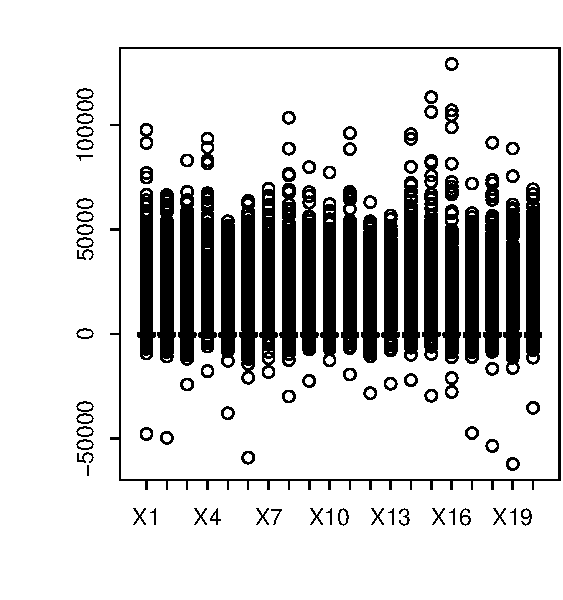
\includegraphics[width=0.47\textwidth]{figs/key-Boxplots-1} 
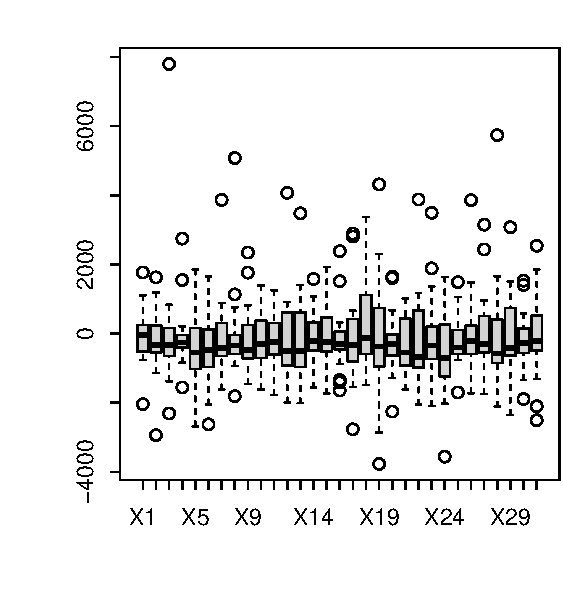
\includegraphics[width=0.47\textwidth]{figs/key-Boxplots-2} 

}


\end{knitrout}
\caption{Boxplots of distributions across features for a selection of observations}
\end{figure}

\begin{knitrout}
\definecolor{shadecolor}{rgb}{0.969, 0.969, 0.969}\color{fgcolor}\begin{kframe}
\begin{alltt}
\hlcom{## Display distributions for the first 20 observations}
\hlkwd{boxplot}\hlstd{(}\hlkwd{data.frame}\hlstd{(GolubB[,} \hlnum{1}\hlopt{:}\hlnum{20}\hlstd{]))}  \hlcom{# First 20 columns (observations)}
\hlcom{## Random selection of 20 rows (features)}
\hlkwd{boxplot}\hlstd{(}\hlkwd{data.frame}\hlstd{(GolubB[}\hlkwd{sample}\hlstd{(}\hlnum{1}\hlopt{:}\hlnum{7129}\hlstd{,} \hlnum{20}\hlstd{), ]))}
\end{alltt}
\end{kframe}
\end{knitrout}

\section{Linear Discriminant Analysis, following variable selection}

\subsection*{Flawed graphs}

Panel A in Figure \ref{fig:biased} shows a convincing separation between
groups, based on the use of linear discriminant analysis with the 15 features
that best separate the groups.  Panel B, which uses random normal data to repeat 
the calculations for Panel A, highlights the flaws in the methodology.



\begin{figure}[h]
\begin{knitrout}
\definecolor{shadecolor}{rgb}{0.969, 0.969, 0.969}\color{fgcolor}

{\centering 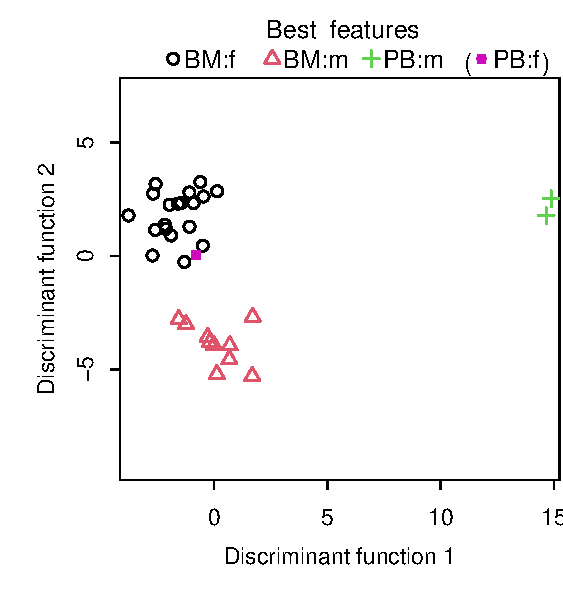
\includegraphics[width=0.47\textwidth]{figs/key-misleading-plots-1} 
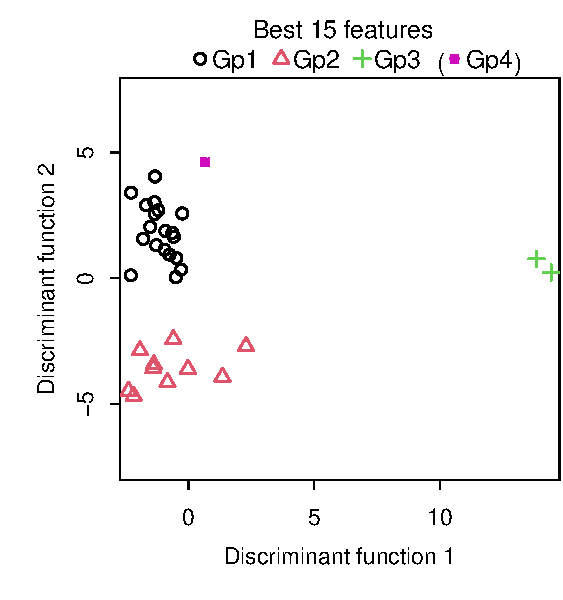
\includegraphics[width=0.47\textwidth]{figs/key-misleading-plots-2} 

}


\end{knitrout}
\caption{Panel B, with random normal data, illustrates the potential for
getting spurious results with the methodology used for Panel A.}\label{fig:biased}
\end{figure}

\begin{knitrout}
\definecolor{shadecolor}{rgb}{0.969, 0.969, 0.969}\color{fgcolor}\begin{kframe}
\begin{alltt}
\hlcom{## Uses orderFeatures() (hddplot); see below}
\hlstd{ord15} \hlkwb{<-} \hlkwd{orderFeatures}\hlstd{(GolubB,} \hlkwc{cl}\hlstd{=tissue.mfB)[}\hlnum{1}\hlopt{:}\hlnum{15}\hlstd{]}
\hlcom{## Panel A}
\hlstd{dfB.ord} \hlkwb{<-} \hlkwd{data.frame}\hlstd{(}\hlkwd{t}\hlstd{(GolubB[ord15, ]))}
\hlcom{## Calculations for the left panel}
\hlcom{## Transpose to observations by features}
\hlstd{dfB15} \hlkwb{<-} \hlkwd{data.frame}\hlstd{(}\hlkwd{t}\hlstd{(GolubB[ord15, ]))}
\hlkwd{library}\hlstd{(MASS)}
\hlstd{dfB15.lda} \hlkwb{<-}  \hlkwd{lda}\hlstd{(dfB15,} \hlkwc{grouping}\hlstd{=tissue.mfB)}
\hlstd{scores} \hlkwb{<-} \hlkwd{predict}\hlstd{(dfB15.lda,} \hlkwc{dimen}\hlstd{=}\hlnum{2}\hlstd{)}\hlopt{$}\hlstd{x}
\hlcom{## Scores for the single PB:f observation}
\hlstd{df.PBf} \hlkwb{<-} \hlkwd{with}\hlstd{(golubInfo,}
  \hlkwd{data.frame}\hlstd{(}\hlkwd{t}\hlstd{(Golub[ord15, tissue.mf}\hlopt{==}\hlstr{"PB:f"} \hlopt{&} \hlstd{cancer}\hlopt{==}\hlstr{"allB"}\hlstd{,}
                     \hlkwc{drop}\hlstd{=}\hlnum{FALSE}\hlstd{])))}
\hlstd{scores.PBf} \hlkwb{<-} \hlkwd{predict}\hlstd{(dfB15.lda,} \hlkwc{newdata}\hlstd{=df.PBf,} \hlkwc{dimen}\hlstd{=}\hlnum{2}\hlstd{)}\hlopt{$}\hlstd{x}
\hlcom{## For comparison: simulated scores}
\hlstd{simscores} \hlkwb{<-} \hlkwd{simulateScores}\hlstd{(}\hlkwc{nrow}\hlstd{=}\hlnum{7129}\hlstd{,} \hlkwc{cl}\hlstd{=}\hlkwd{rep}\hlstd{(}\hlnum{1}\hlopt{:}\hlnum{3}\hlstd{,} \hlkwd{c}\hlstd{(}\hlnum{19}\hlstd{,}\hlnum{10}\hlstd{,}\hlnum{2}\hlstd{)),}
                            \hlkwc{cl.other}\hlstd{=}\hlnum{4}\hlstd{,} \hlkwc{nfeatures}\hlstd{=}\hlnum{15}\hlstd{,} \hlkwc{seed}\hlstd{=}\hlnum{41}\hlstd{)}
  \hlcom{# Returns list elements: scores, cl, scores.other & cl.other}
\end{alltt}
\end{kframe}
\end{knitrout}

\begin{knitrout}
\definecolor{shadecolor}{rgb}{0.969, 0.969, 0.969}\color{fgcolor}\begin{kframe}
\begin{alltt}
\hlstd{opar} \hlkwb{<-} \hlkwd{par}\hlstd{(}\hlkwc{mar}\hlstd{=}\hlkwd{c}\hlstd{(}\hlnum{4}\hlstd{,}\hlnum{4}\hlstd{,}\hlnum{2.6}\hlstd{,}\hlnum{.1}\hlstd{))}
\hlcom{## Warning! The plot that now follows may be misleading!}
\hlcom{## Use scoreplot(), from the hddplot package}
\hlkwd{scoreplot}\hlstd{(}\hlkwd{list}\hlstd{(}\hlkwc{scores}\hlstd{=scores,} \hlkwc{cl}\hlstd{=tissue.mfB,} \hlkwc{other}\hlstd{=scores.PBf,}
               \hlkwc{cl.other}\hlstd{=}\hlstr{"PB:f"}\hlstd{))}
\hlcom{## Panel B: Repeat plot, now with random normal data}
\hlkwd{scoreplot}\hlstd{(simscores)}
\hlkwd{par}\hlstd{(opar)}
\end{alltt}
\end{kframe}
\end{knitrout}

\section{Distributional extremes}

Calculated F-statistics (Figure \ref{fig:qq}) will be compared with 
the permutation distribution and with the theoretical F-distribution,
but limiting attention to just the first two classes.  At least in
version 2.56.0 of \texttt{multtest}, calculations fail if the minimum
class size is 1 or 2, as for \texttt{PB:m}. Code is:

\begin{knitrout}
\definecolor{shadecolor}{rgb}{0.969, 0.969, 0.969}\color{fgcolor}\begin{kframe}
\begin{alltt}
\hlcom{## In the following, B is too small for the simulation to give a}
\hlcom{## good indication of behavior in the extreme tail.}
\hlkwd{library}\hlstd{(multtest,} \hlkwc{quietly}\hlstd{=}\hlnum{TRUE}\hlstd{)}
\hlstd{GolubB2} \hlkwb{<-} \hlstd{GolubB[,tissue.mfB}\hlopt{!=}\hlstr{"PB:m"}\hlstd{]}
\hlstd{cl.mfB2} \hlkwb{<-}  \hlstd{(}\hlkwd{unclass}\hlstd{(tissue.mfB)}\hlopt{-}\hlnum{1}\hlstd{)[tissue.mfB}\hlopt{!=}\hlstr{"PB:m"}\hlstd{]}
\hlstd{GolubB.maxT} \hlkwb{<-} \hlkwd{mt.maxT}\hlstd{(GolubB2, cl.mfB2,} \hlkwc{test}\hlstd{=}\hlstr{"f"}\hlstd{,} \hlkwc{B}\hlstd{=}\hlnum{1000}\hlstd{)}
\end{alltt}
\end{kframe}
\end{knitrout}

\begin{knitrout}
\definecolor{shadecolor}{rgb}{0.969, 0.969, 0.969}\color{fgcolor}\begin{kframe}
\begin{alltt}
\hlcom{## Compare calculated F-statistics with permutation distribution}
\hlkwd{qqthin}\hlstd{(}\hlkwd{qf}\hlstd{(}\hlnum{1}\hlopt{-}\hlstd{GolubB.maxT}\hlopt{$}\hlstd{rawp,} \hlnum{2}\hlstd{,} \hlnum{28}\hlstd{), GolubB.maxT}\hlopt{$}\hlstd{teststat,}
       \hlkwc{print.thinning.details} \hlstd{=} \hlnum{FALSE}\hlstd{)}
\hlcom{## Compare calculated F-statistics with theoretical F-distribution}
\hlkwd{qqthin}\hlstd{(}\hlkwd{qf}\hlstd{(}\hlkwd{ppoints}\hlstd{(}\hlnum{7129}\hlstd{),} \hlnum{2}\hlstd{,} \hlnum{28}\hlstd{), GolubB.maxT}\hlopt{$}\hlstd{teststat,}
       \hlkwc{print.thinning.details} \hlstd{=} \hlnum{FALSE}\hlstd{)}
  \hlcom{# The theoretical F-distribution gives estimates of quantiles}
  \hlcom{# that are too small}
\hlcom{## NB also the comparison between the permutation distribution}
\hlcom{## and the theoretical F:}
\hlkwd{qqthin}\hlstd{(}\hlkwd{qf}\hlstd{(}\hlkwd{ppoints}\hlstd{(}\hlnum{7129}\hlstd{),} \hlnum{2}\hlstd{,} \hlnum{28}\hlstd{),} \hlkwd{qf}\hlstd{(}\hlnum{1}\hlopt{-}\hlstd{GolubB.maxT}\hlopt{$}\hlstd{rawp,} \hlnum{2}\hlstd{,} \hlnum{28}\hlstd{),}
       \hlkwc{print.thinning.details} \hlstd{=} \hlnum{FALSE}\hlstd{)}
  \hlcom{# qqthin() is a version of qqplot() that thins out points where}
  \hlcom{# overlap is substantial, thus giving smaller graphics files.}
\end{alltt}
\end{kframe}
\end{knitrout}

\begin{figure}
\begin{knitrout}
\definecolor{shadecolor}{rgb}{0.969, 0.969, 0.969}\color{fgcolor}

{\centering 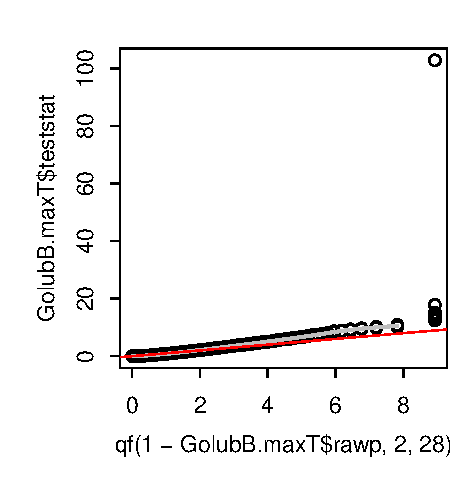
\includegraphics[width=0.32\textwidth]{figs/key-plot-Fstats-1} 
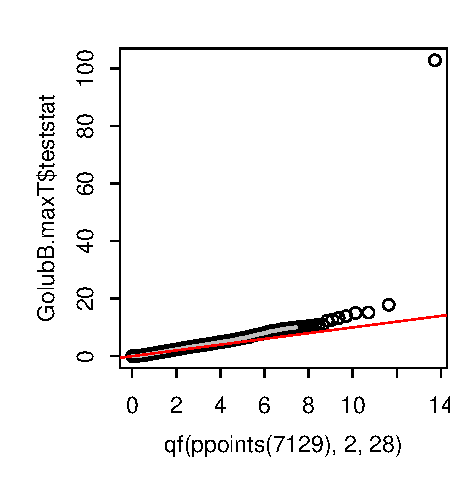
\includegraphics[width=0.32\textwidth]{figs/key-plot-Fstats-2} 
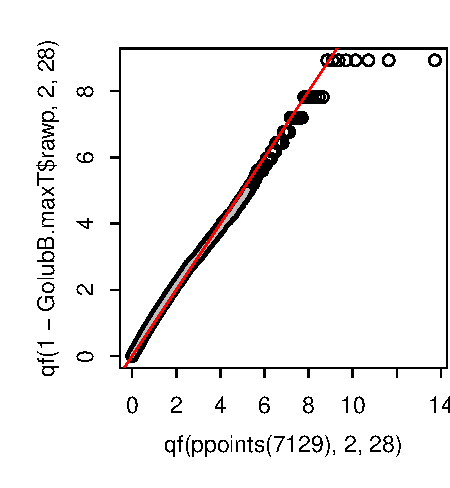
\includegraphics[width=0.32\textwidth]{figs/key-plot-Fstats-3} 

}


\end{knitrout}
\caption{Compare calculated F-statistics with the permutation distribution 
and with the theoretical F. The theoretical F makes unrealistic normality 
and independence assumptions.}\label{fig:qq}
\end{figure}

\begin{knitrout}
\definecolor{shadecolor}{rgb}{0.969, 0.969, 0.969}\color{fgcolor}\begin{kframe}
\begin{alltt}
\hlcom{## In the following, B is too small for the simulation to give a}
\hlcom{## good indication of behavior in the extreme tail.}
\hlkwd{library}\hlstd{(multtest,} \hlkwc{quietly}\hlstd{=}\hlnum{TRUE}\hlstd{)}
\hlstd{GolubB2} \hlkwb{<-} \hlstd{GolubB[,tissue.mfB}\hlopt{!=}\hlstr{"PB:m"}\hlstd{]}
\hlstd{cl.mfB2} \hlkwb{<-}  \hlstd{(}\hlkwd{unclass}\hlstd{(tissue.mfB)}\hlopt{-}\hlnum{1}\hlstd{)[tissue.mfB}\hlopt{!=}\hlstr{"PB:m"}\hlstd{]}
\hlstd{GolubB.maxT} \hlkwb{<-} \hlkwd{mt.maxT}\hlstd{(GolubB2, cl.mfB2,} \hlkwc{test}\hlstd{=}\hlstr{"f"}\hlstd{,} \hlkwc{B}\hlstd{=}\hlnum{1000}\hlstd{)}
\end{alltt}
\end{kframe}
\end{knitrout}

\begin{knitrout}
\definecolor{shadecolor}{rgb}{0.969, 0.969, 0.969}\color{fgcolor}\begin{kframe}
\begin{alltt}
\hlcom{## Compare calculated F-statistics with permutation distribution}
\hlkwd{qqthin}\hlstd{(}\hlkwd{qf}\hlstd{(}\hlnum{1}\hlopt{-}\hlstd{GolubB.maxT}\hlopt{$}\hlstd{rawp,} \hlnum{2}\hlstd{,} \hlnum{28}\hlstd{), GolubB.maxT}\hlopt{$}\hlstd{teststat,}
       \hlkwc{print.thinning.details} \hlstd{=} \hlnum{FALSE}\hlstd{)}
\hlcom{## Compare calculated F-statistics with theoretical F-distribution}
\hlkwd{qqthin}\hlstd{(}\hlkwd{qf}\hlstd{(}\hlkwd{ppoints}\hlstd{(}\hlnum{7129}\hlstd{),} \hlnum{2}\hlstd{,} \hlnum{28}\hlstd{), GolubB.maxT}\hlopt{$}\hlstd{teststat,}
       \hlkwc{print.thinning.details} \hlstd{=} \hlnum{FALSE}\hlstd{)}
  \hlcom{# The theoretical F-distribution gives estimates of quantiles}
  \hlcom{# that are too small}
\hlcom{## NB also the comparison between the permutation distribution}
\hlcom{## and the theoretical F:}
\hlkwd{qqthin}\hlstd{(}\hlkwd{qf}\hlstd{(}\hlkwd{ppoints}\hlstd{(}\hlnum{7129}\hlstd{),} \hlnum{2}\hlstd{,} \hlnum{28}\hlstd{),} \hlkwd{qf}\hlstd{(}\hlnum{1}\hlopt{-}\hlstd{GolubB.maxT}\hlopt{$}\hlstd{rawp,} \hlnum{2}\hlstd{,} \hlnum{28}\hlstd{),}
       \hlkwc{print.thinning.details} \hlstd{=} \hlnum{FALSE}\hlstd{)}
  \hlcom{# qqthin() is a version of qqplot() that thins out points where}
  \hlcom{# overlap is substantial, thus giving smaller graphics files.}
\end{alltt}
\end{kframe}
\end{knitrout}

\section{Discriminant Analysis -- Training/Test}
\begin{knitrout}
\definecolor{shadecolor}{rgb}{0.969, 0.969, 0.969}\color{fgcolor}\begin{kframe}
\begin{alltt}
\hlcom{##              Selection of features that discriminate}
\hlcom{## ss 12.3.3: Accuracies and Scores for test data}
\hlstd{Golub.BM} \hlkwb{<-} \hlkwd{with}\hlstd{(golubInfo, Golub[, BM.PB}\hlopt{==}\hlstr{"BM"}\hlstd{])}
\hlstd{cancer.BM} \hlkwb{<-} \hlkwd{with}\hlstd{(golubInfo, cancer[BM.PB}\hlopt{==}\hlstr{"BM"}\hlstd{])}
\hlcom{## Now split each of the cancer.BM categories between two subsets}
\hlcom{##  Uses divideUp(), from hddplot}
\hlstd{gp.id} \hlkwb{<-} \hlkwd{divideUp}\hlstd{(cancer.BM,} \hlkwc{nset}\hlstd{=}\hlnum{2}\hlstd{,} \hlkwc{seed}\hlstd{=}\hlnum{29}\hlstd{)}
  \hlcom{# Set seed to allow exact reproduction of the results below}
\hlkwd{table}\hlstd{(gp.id, cancer.BM)}
\end{alltt}
\begin{verbatim}
     cancer.BM
gp.id allB allT aml
    1   17    4  10
    2   16    4  11
\end{verbatim}
\end{kframe}
\end{knitrout}

\begin{knitrout}
\definecolor{shadecolor}{rgb}{0.969, 0.969, 0.969}\color{fgcolor}\begin{kframe}
\begin{alltt}
\hlstd{accboth} \hlkwb{<-} \hlkwd{accTrainTest}\hlstd{(}\hlkwc{x} \hlstd{= Golub.BM,} \hlkwc{cl} \hlstd{= cancer.BM,}
                        \hlkwc{traintest}\hlstd{=gp.id, ,} \hlkwc{print.progress}\hlstd{=}\hlnum{FALSE}\hlstd{)}
\end{alltt}
\begin{verbatim}

                                                      
Training/test split          Best accuracy, less 1SD  
I (training) / II (test)     0.89 (14 features)       
II (training) / I (test)     0.92 (10 features)       
                                               
Training/test split          Best accuracy     
I (training) / II (test)     0.94 (20 features)
II (training) / I (test)     0.97 (17 features)
\end{verbatim}
\end{kframe}
\end{knitrout}

\begin{figure}[h]
\begin{knitrout}
\definecolor{shadecolor}{rgb}{0.969, 0.969, 0.969}\color{fgcolor}

{\centering 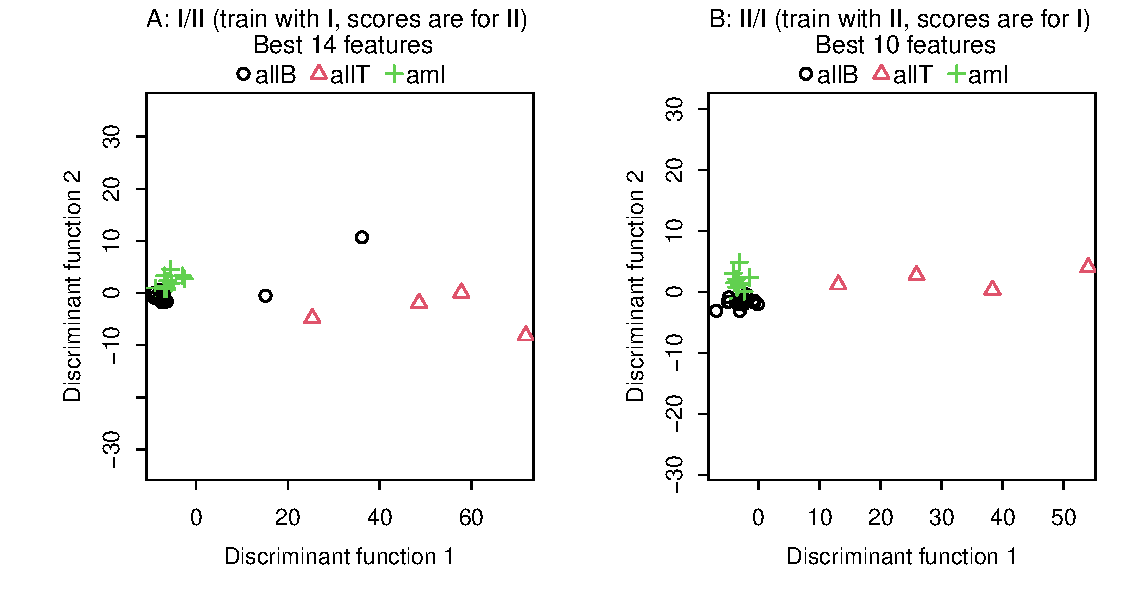
\includegraphics[width=0.97\textwidth]{figs/key-plot-train-test-1} 

}


\end{knitrout}
\caption{Panel A plots scores for the set II data, using set I for
  training (the I/II split), as described in the text. Panel B plots
  the scores for the set I data when the roles of the two sets
  were reversed, i.e., the split was II/I.}
\label{fig:traintest}
\end{figure}

Code for plotting the figures is:
\begin{knitrout}
\definecolor{shadecolor}{rgb}{0.969, 0.969, 0.969}\color{fgcolor}\begin{kframe}
\begin{alltt}
\hlstd{opar} \hlkwb{<-} \hlkwd{par}\hlstd{(}\hlkwc{mar}\hlstd{=}\hlkwd{c}\hlstd{(}\hlnum{4}\hlstd{,}\hlnum{4}\hlstd{,}\hlnum{3.1}\hlstd{,}\hlnum{.1}\hlstd{))}
\hlcom{## Use function plotTrainTest() from hddplot}
\hlkwd{plotTrainTest}\hlstd{(}\hlkwc{x}\hlstd{=Golub.BM,} \hlkwc{nfeatures}\hlstd{=}\hlkwd{c}\hlstd{(}\hlnum{14}\hlstd{,}\hlnum{10}\hlstd{),} \hlkwc{cl}\hlstd{=cancer.BM,} \hlkwc{traintest}\hlstd{=gp.id)}
\hlkwd{par}\hlstd{(opar)}
\end{alltt}
\end{kframe}
\end{knitrout}

Now compare the choice of features between I/II and II/I:
\begin{knitrout}
\definecolor{shadecolor}{rgb}{0.969, 0.969, 0.969}\color{fgcolor}\begin{kframe}
\begin{alltt}
\hlkwd{rbind}\hlstd{(accboth}\hlopt{$}\hlstd{sub1.2[}\hlnum{1}\hlopt{:}\hlnum{20}\hlstd{],accboth}\hlopt{$}\hlstd{sub2.1[}\hlnum{1}\hlopt{:}\hlnum{20}\hlstd{])}
\end{alltt}
\begin{verbatim}
     [,1] [,2] [,3] [,4] [,5] [,6] [,7] [,8] [,9] [,10] [,11] [,12]
[1,] 4050 2794 6510 6696 4342 5542 4357 5543 1207  4584  6236  1429
[2,] 6606 4342 6510 3594 4050 6236 1694 1207 1268  4847  5542  2061
     [,13] [,14] [,15] [,16] [,17] [,18] [,19] [,20]
[1,]  6575  2833  4750  2335  1704  4882  6225  3544
[2,]  5543  4055  4375  1144   379  6696  4196   229
\end{verbatim}
\begin{alltt}
\hlkwd{match}\hlstd{(accboth}\hlopt{$}\hlstd{sub1.2[}\hlnum{1}\hlopt{:}\hlnum{20}\hlstd{],accboth}\hlopt{$}\hlstd{sub2.1[}\hlnum{1}\hlopt{:}\hlnum{20}\hlstd{])}
\end{alltt}
\begin{verbatim}
 [1]  5 NA  3 18  2 11 NA 13  8 NA  6 NA NA NA NA NA NA NA NA NA
\end{verbatim}
\end{kframe}
\end{knitrout}

\subsection{Cross-validation based optimum choice of features}

With the number of selected features varying from 1 to 25, 
three different accuracy measures will be compared, for
classification of the B-cell data. The plots highlight the
serious bias in measures that are to an extent internal to
the training data.

\begin{knitrout}
\definecolor{shadecolor}{rgb}{0.969, 0.969, 0.969}\color{fgcolor}\begin{kframe}
\begin{alltt}
\hlcom{##  Cross-validation to determine the optimum number of features}
\hlcom{## Accuracy measure will be: tissue.mfB.cv$acc.cv}
\hlstd{tissue.mfB.cv} \hlkwb{<-} \hlkwd{cvdisc}\hlstd{(GolubB,} \hlkwc{cl}\hlstd{=tissue.mfB,} \hlkwc{nfeatures}\hlstd{=}\hlnum{1}\hlopt{:}\hlnum{23}\hlstd{,}
                        \hlkwc{nfold}\hlstd{=}\hlkwd{c}\hlstd{(}\hlnum{5}\hlstd{,}\hlnum{1}\hlstd{),} \hlkwc{print.progress}\hlstd{=}\hlnum{FALSE}\hlstd{)}
\end{alltt}
\begin{verbatim}

                                                              
Accuracy           Best accuracy, less 1SD   Best accuracy    
(Cross-validation) 0.77 (3 features)         0.84 (7 features)
\end{verbatim}
\begin{alltt}
  \hlcom{# 5-fold CV (x1)}
\hlcom{## Defective measures will be in acc.resub (resubstitution)}
\hlcom{## and acc.sel1 (select features prior to cross-validation)}
\hlstd{tissue.mfB.badcv} \hlkwb{<-} \hlkwd{defectiveCVdisc}\hlstd{(GolubB,} \hlkwc{cl}\hlstd{=tissue.mfB,}
                                   \hlkwc{foldids}\hlstd{=tissue.mfB.cv}\hlopt{$}\hlstd{folds,}
                                   \hlkwc{nfeatures}\hlstd{=}\hlnum{1}\hlopt{:}\hlnum{23}\hlstd{,} \hlkwc{nfold}\hlstd{=}\hlkwd{c}\hlstd{(}\hlnum{5}\hlstd{,}\hlnum{1}\hlstd{),}
                                   \hlkwc{print.progress}\hlstd{=}\hlnum{FALSE}\hlstd{)}
\hlcom{## NB: Warning messages have been omitted}
\end{alltt}
\end{kframe}
\end{knitrout}

\begin{knitrout}
\definecolor{shadecolor}{rgb}{0.969, 0.969, 0.969}\color{fgcolor}\begin{kframe}
\begin{alltt}
\hlcom{## Calculations for random normal data:}
\hlkwd{set.seed}\hlstd{(}\hlnum{43}\hlstd{)}
\hlstd{rGolubB} \hlkwb{<-} \hlkwd{matrix}\hlstd{(}\hlkwd{rnorm}\hlstd{(}\hlkwd{prod}\hlstd{(}\hlkwd{dim}\hlstd{(GolubB))),} \hlkwc{nrow}\hlstd{=}\hlkwd{dim}\hlstd{(GolubB)[}\hlnum{1}\hlstd{])}
\hlstd{rtissue.mfB.cv} \hlkwb{<-} \hlkwd{cvdisc}\hlstd{(rGolubB,} \hlkwc{cl}\hlstd{=tissue.mfB,} \hlkwc{nfeatures}\hlstd{=}\hlnum{1}\hlopt{:}\hlnum{23}\hlstd{,}
                         \hlkwc{nfold}\hlstd{=}\hlkwd{c}\hlstd{(}\hlnum{5}\hlstd{,}\hlnum{1}\hlstd{),} \hlkwc{print.progress}\hlstd{=}\hlnum{FALSE}\hlstd{)}
\end{alltt}
\begin{verbatim}
[1] "Input rows (features) are not named. Names"
[1] "1:7129 will be assigned."

                                                              
Accuracy           Best accuracy, less 1SD   Best accuracy    
(Cross-validation) 0.46 (1 features)         0.55 (1 features)
\end{verbatim}
\begin{alltt}
\hlstd{rtissue.mfB.badcv} \hlkwb{<-} \hlkwd{defectiveCVdisc}\hlstd{(rGolubB,} \hlkwc{cl}\hlstd{=tissue.mfB,}
                                   \hlkwc{nfeatures}\hlstd{=}\hlnum{1}\hlopt{:}\hlnum{23}\hlstd{,} \hlkwc{nfold}\hlstd{=}\hlkwd{c}\hlstd{(}\hlnum{5}\hlstd{,}\hlnum{1}\hlstd{),}
                                   \hlkwc{foldids}\hlstd{=rtissue.mfB.cv}\hlopt{$}\hlstd{folds,}
                                   \hlkwc{print.progress}\hlstd{=}\hlnum{FALSE}\hlstd{)}
\end{alltt}
\begin{verbatim}
[1] "Input rows (features) are not named. Names"
[1] "1:7129 will be assigned."
\end{verbatim}
\end{kframe}
\end{knitrout}

\begin{knitrout}
\definecolor{shadecolor}{rgb}{0.969, 0.969, 0.969}\color{fgcolor}\begin{kframe}
\begin{alltt}
\hlcom{## This function will be used for the plots}
\hlstd{plot.acc} \hlkwb{<-} \hlkwa{function}\hlstd{(}\hlkwc{cv}\hlstd{=cv1,} \hlkwc{badcv}\hlstd{=badcv1,} \hlkwc{nseq}\hlstd{=}\hlkwa{NULL}\hlstd{,} \hlkwc{badnseq}\hlstd{=}\hlkwa{NULL}\hlstd{,}
                     \hlkwc{title}\hlstd{=}\hlstr{""}\hlstd{,} \hlkwc{ylab}\hlstd{=}\hlstr{"Predictive accuracy"}\hlstd{,}
                     \hlkwc{add.legend}\hlstd{=}\hlnum{TRUE}\hlstd{)\{}
  \hlstd{maxg} \hlkwb{<-} \hlkwd{min}\hlstd{(}\hlkwd{c}\hlstd{(}\hlkwd{length}\hlstd{(badcv}\hlopt{$}\hlstd{acc.resub),} \hlkwd{length}\hlstd{(cv}\hlopt{$}\hlstd{acc.cv)))}
  \hlkwa{if}\hlstd{(}\hlkwd{is.null}\hlstd{(nseq))nseq} \hlkwb{<-} \hlnum{1}\hlopt{:}\hlstd{maxg}
  \hlkwd{plot}\hlstd{(nseq, badcv}\hlopt{$}\hlstd{acc.resub[}\hlnum{1}\hlopt{:}\hlstd{maxg],} \hlkwc{ylim}\hlstd{=}\hlkwd{c}\hlstd{(}\hlnum{0}\hlstd{,}\hlnum{1}\hlstd{),} \hlkwc{type}\hlstd{=}\hlstr{"n"}\hlstd{,}
       \hlkwc{yaxs}\hlstd{=}\hlstr{"i"}\hlstd{,} \hlkwc{xlab}\hlstd{=}\hlstr{"Number of features selected"}\hlstd{,} \hlkwc{ylab}\hlstd{=ylab)}
  \hlkwd{par}\hlstd{(}\hlkwc{xpd}\hlstd{=T)}
  \hlkwd{points}\hlstd{(nseq, badcv}\hlopt{$}\hlstd{acc.resub[}\hlnum{1}\hlopt{:}\hlstd{maxg],} \hlkwc{col}\hlstd{=}\hlnum{2}\hlstd{,} \hlkwc{type}\hlstd{=}\hlstr{"b"}\hlstd{,} \hlkwc{lty}\hlstd{=}\hlnum{2}\hlstd{,}
         \hlkwc{pch}\hlstd{=}\hlnum{0}\hlstd{,} \hlkwc{cex}\hlstd{=}\hlnum{0.8}\hlstd{)}
  \hlkwd{par}\hlstd{(}\hlkwc{xpd}\hlstd{=}\hlnum{FALSE}\hlstd{)}
  \hlkwd{points}\hlstd{(nseq, badcv}\hlopt{$}\hlstd{acc.sel1[}\hlnum{1}\hlopt{:}\hlstd{maxg],} \hlkwc{col}\hlstd{=}\hlstr{"gray40"}\hlstd{,} \hlkwc{pch}\hlstd{=}\hlnum{3}\hlstd{,} \hlkwc{cex}\hlstd{=}\hlnum{0.8}\hlstd{)}
  \hlkwd{lines}\hlstd{(}\hlkwd{lowess}\hlstd{(nseq, badcv}\hlopt{$}\hlstd{acc.sel1[}\hlnum{1}\hlopt{:}\hlstd{maxg],} \hlkwc{f}\hlstd{=}\hlnum{.325}\hlstd{,} \hlkwc{iter}\hlstd{=}\hlnum{0}\hlstd{),}
        \hlkwc{col}\hlstd{=}\hlstr{"gray40"}\hlstd{,} \hlkwc{lty}\hlstd{=}\hlnum{2}\hlstd{)}
  \hlkwd{points}\hlstd{(nseq, cv}\hlopt{$}\hlstd{acc.cv[}\hlnum{1}\hlopt{:}\hlstd{maxg],} \hlkwc{col}\hlstd{=}\hlstr{"blue"}\hlstd{,} \hlkwc{pch}\hlstd{=}\hlnum{1}\hlstd{,} \hlkwc{cex}\hlstd{=}\hlnum{0.8}\hlstd{)}
  \hlkwd{lines}\hlstd{(}\hlkwd{lowess}\hlstd{(nseq, cv}\hlopt{$}\hlstd{acc.cv[}\hlnum{1}\hlopt{:}\hlstd{maxg],} \hlkwc{f}\hlstd{=}\hlnum{.325}\hlstd{,} \hlkwc{iter}\hlstd{=}\hlnum{0}\hlstd{),} \hlkwc{col}\hlstd{=}\hlstr{"blue"}\hlstd{,}
        \hlkwc{lwd}\hlstd{=}\hlnum{2}\hlstd{)}
  \hlstd{xy} \hlkwb{<-} \hlkwd{par}\hlstd{()}\hlopt{$}\hlstd{usr[}\hlkwd{c}\hlstd{(}\hlnum{1}\hlstd{,}\hlnum{3}\hlstd{)]}
  \hlkwa{if}\hlstd{(add.legend)}
    \hlkwd{legend}\hlstd{(xy[}\hlnum{1}\hlstd{], xy[}\hlnum{2}\hlstd{],} \hlkwc{xjust}\hlstd{=}\hlnum{0}\hlstd{,} \hlkwc{yjust}\hlstd{=}\hlnum{0}\hlstd{,}
           \hlkwc{legend}\hlstd{=}\hlkwd{c}\hlstd{(}\hlstr{"Training set 'accuracy'"}\hlstd{,}
             \hlstr{"Defective cross-validation"}\hlstd{,}
             \hlstr{"Cross-validation - select at each fold"}\hlstd{),}
           \hlkwc{lty}\hlstd{=}\hlkwd{c}\hlstd{(}\hlnum{1}\hlstd{,}\hlnum{2}\hlstd{,}\hlnum{1}\hlstd{),} \hlkwc{lwd}\hlstd{=}\hlkwd{c}\hlstd{(}\hlnum{1}\hlstd{,}\hlnum{1}\hlstd{,}\hlnum{2}\hlstd{),} \hlkwc{pch}\hlstd{=}\hlkwd{c}\hlstd{(}\hlnum{0}\hlstd{,}\hlnum{3}\hlstd{,}\hlnum{1}\hlstd{),}
           \hlkwc{col}\hlstd{=}\hlkwd{c}\hlstd{(}\hlstr{"red"}\hlstd{,}\hlstr{"gray40"}\hlstd{,}\hlstr{"blue"}\hlstd{),} \hlkwc{cex}\hlstd{=}\hlnum{0.875}\hlstd{)}
  \hlkwd{mtext}\hlstd{(}\hlkwc{side}\hlstd{=}\hlnum{3}\hlstd{,}\hlkwc{line}\hlstd{=}\hlnum{0.35}\hlstd{, title,} \hlkwc{adj}\hlstd{=}\hlnum{0}\hlstd{)}
\hlstd{\}}
\end{alltt}
\end{kframe}
\end{knitrout}

\begin{figure}[h]
\begin{knitrout}
\definecolor{shadecolor}{rgb}{0.969, 0.969, 0.969}\color{fgcolor}\begin{kframe}
\begin{alltt}
\hlkwd{plot.acc}\hlstd{(tissue.mfB.cv, tissue.mfB.badcv,}
         \hlkwc{title}\hlstd{=}\hlstr{"A: Golub data (as for Figure 12.9)"}\hlstd{)}
\hlkwd{plot.acc}\hlstd{(rtissue.mfB.cv, rtissue.mfB.badcv,} \hlkwc{ylab}\hlstd{=}\hlstr{""}\hlstd{,}
         \hlkwc{title}\hlstd{=}\hlstr{"B: Random data"}\hlstd{,} \hlkwc{add.legend}\hlstd{=}\hlnum{FALSE}\hlstd{)}
\end{alltt}
\end{kframe}

{\centering 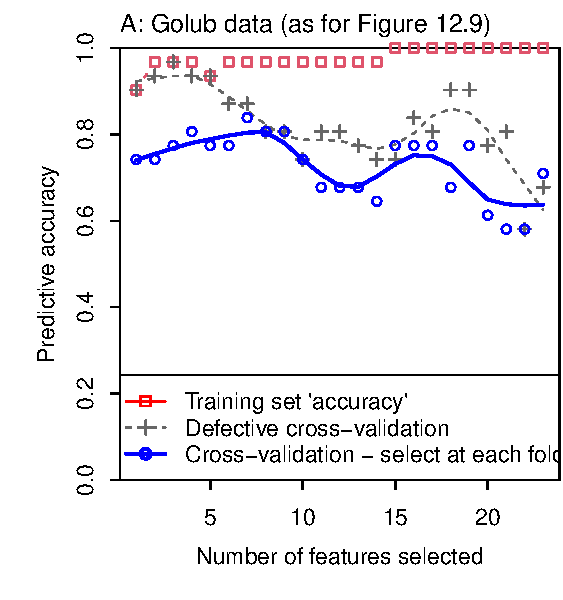
\includegraphics[width=0.47\textwidth]{figs/key-cv-bad-1} 
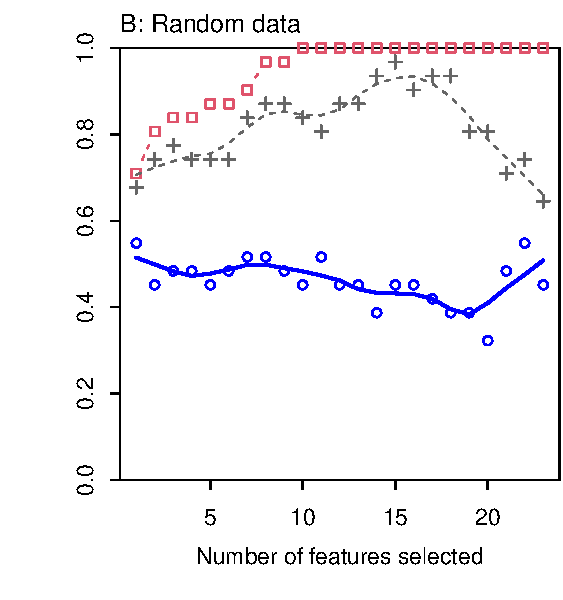
\includegraphics[width=0.47\textwidth]{figs/key-cv-bad-2} 

}


\end{knitrout}
\caption{Comparison of different accuracy measures, in the development
  of a discriminant rule for the classification, into the categories
  \texttt{BM:f}, \texttt{BM:m} and \texttt{PB:m}, of the B-cell ALL
  data for which gender is known.}\label{fig:cv-acc}

\end{figure}

Figure \ref{fig:cv-acc} compares three different accuracy measures, for
the classification of the B-cell data.  The training data measure ($\Box$)
  is a severely biased measure.  Cross-validation, but with features
  selected using all the data ($+$), is less severely biased.  An
  acceptable measure of predictive accuracy ($\circ$) requires
  re-selection of features at each fold of the cross-validation.  The
  right panel shows the performance of each of these measures when the
  expression values were replaced by random data.

\subsection*{Which features?}
\begin{knitrout}
\definecolor{shadecolor}{rgb}{0.969, 0.969, 0.969}\color{fgcolor}\begin{kframe}
\begin{alltt}
\hlcom{##                          Which features?}
\hlstd{genelist} \hlkwb{<-} \hlkwd{matrix}\hlstd{(tissue.mfB.cv}\hlopt{$}\hlstd{genelist[}\hlnum{1}\hlopt{:}\hlnum{3}\hlstd{, ,],} \hlkwc{nrow}\hlstd{=}\hlnum{3}\hlstd{)}
\hlstd{tab} \hlkwb{<-} \hlkwd{table}\hlstd{(genelist,} \hlkwd{row}\hlstd{(genelist))}
\hlstd{ord} \hlkwb{<-} \hlkwd{order}\hlstd{(tab[,}\hlnum{1}\hlstd{], tab[,}\hlnum{2}\hlstd{],} \hlkwc{decreasing}\hlstd{=}\hlnum{TRUE}\hlstd{)}
\hlstd{tab[ord,]}
\end{alltt}
\begin{verbatim}
                
genelist         1 2 3
  M58459_at      3 0 1
  L08666_at      1 0 0
  U29195_at      1 0 0
  U91327_at      0 2 0
  U49395_at      0 1 0
  X00437_s_at    0 1 0
  X54870_at      0 1 0
  X62654_rna1_at 0 0 3
  X82494_at      0 0 1
\end{verbatim}
\end{kframe}
\end{knitrout}


\section{Cross-validation: bone marrow (\texttt{BM}) samples}
\begin{knitrout}
\definecolor{shadecolor}{rgb}{0.969, 0.969, 0.969}\color{fgcolor}\begin{kframe}
\begin{alltt}
\hlcom{##         Cross-validation: bone marrow (\{BM\}) samples only}
\hlstd{BMonly.cv} \hlkwb{<-} \hlkwd{cvdisc}\hlstd{(Golub.BM,} \hlkwc{cl}\hlstd{=cancer.BM,} \hlkwc{nfeatures}\hlstd{=}\hlnum{1}\hlopt{:}\hlnum{25}\hlstd{,}
                    \hlkwc{nfold}\hlstd{=}\hlkwd{c}\hlstd{(}\hlnum{5}\hlstd{,}\hlnum{1}\hlstd{),} \hlkwc{print.progress}\hlstd{=}\hlnum{FALSE}\hlstd{)}
\end{alltt}
\begin{verbatim}

                                                              
Accuracy           Best accuracy, less 1SD   Best accuracy    
(Cross-validation) 0.87 (12 features)        0.9 (16 features)
\end{verbatim}
\begin{alltt}
\hlstd{tissue.mfB.scores} \hlkwb{<-}
  \hlkwd{cvscores}\hlstd{(}\hlkwc{cvlist} \hlstd{= tissue.mfB.cv,} \hlkwc{nfeatures} \hlstd{=} \hlnum{3}\hlstd{,} \hlkwc{cl.other} \hlstd{=} \hlkwa{NULL}\hlstd{,}
           \hlkwc{print.progress}\hlstd{=}\hlnum{FALSE}\hlstd{)}
\end{alltt}
\begin{verbatim}

1:2:3:4:5
\end{verbatim}
\begin{alltt}
\hlstd{BMonly.scores} \hlkwb{<-} \hlkwd{cvscores}\hlstd{(}\hlkwc{cvlist}\hlstd{=BMonly.cv,} \hlkwc{nfeatures}\hlstd{=}\hlnum{19}\hlstd{,}
                          \hlkwc{cl.other}\hlstd{=}\hlkwa{NULL}\hlstd{,} \hlkwc{print.progress}\hlstd{=}\hlnum{FALSE}\hlstd{)}
\end{alltt}
\begin{verbatim}

1:2:3:4:5
\end{verbatim}
\end{kframe}
\end{knitrout}

\begin{figure}
\begin{knitrout}
\definecolor{shadecolor}{rgb}{0.969, 0.969, 0.969}\color{fgcolor}

{\centering 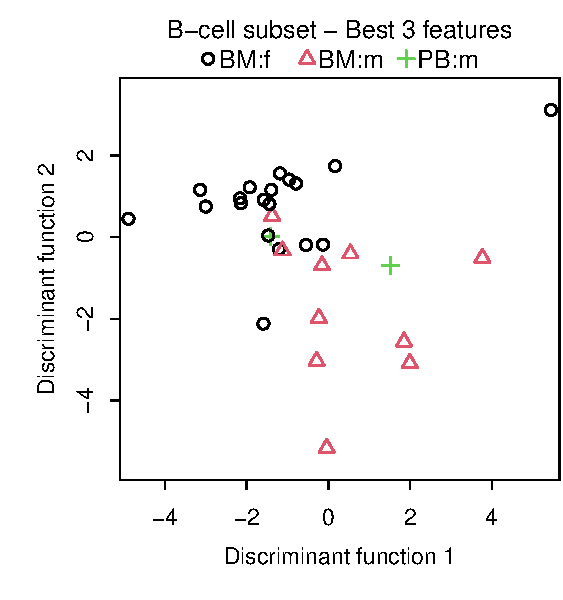
\includegraphics[width=0.47\textwidth]{figs/key-cv-Bcell-gphAB-1} 
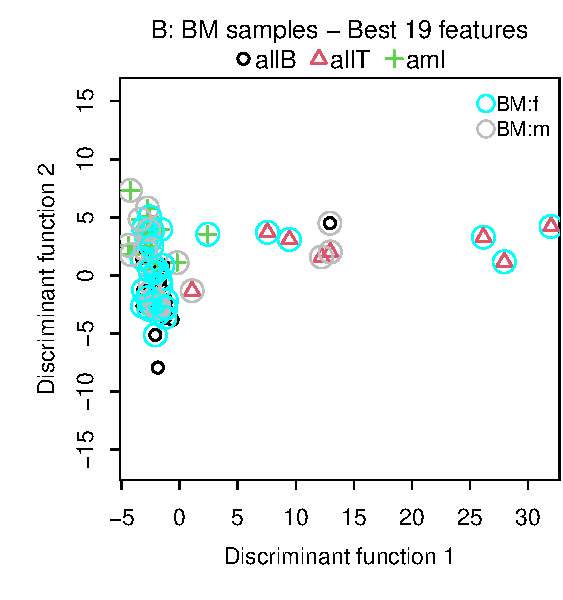
\includegraphics[width=0.47\textwidth]{figs/key-cv-Bcell-gphAB-2} 

}


\end{knitrout}
\caption{These plots of projections of linear discriminant analysis
  scores are designed to fairly reflect the performance of a linear
  discriminant in distinguishing between known groups in the data. The
  two panels relate to different subsets of the \texttt{Golub} data,
  with different groupings in the two cases.  In panel B, for the
  classification of the 62 bone marrow (\texttt{BM}) samples into
  \texttt{allB}, \texttt{allT}, and \texttt{aml}, points where the sex
  is known are identified as male or female.}
\end{figure}

Code is:
\begin{knitrout}
\definecolor{shadecolor}{rgb}{0.969, 0.969, 0.969}\color{fgcolor}\begin{kframe}
\begin{alltt}
\hlstd{opar} \hlkwb{<-} \hlkwd{par}\hlstd{(}\hlkwc{mar}\hlstd{=}\hlkwd{c}\hlstd{(}\hlnum{4}\hlstd{,}\hlnum{4}\hlstd{,}\hlnum{2.6}\hlstd{,}\hlnum{.1}\hlstd{))}
\hlcom{## Panel A: Uses tissue.mfB.acc from above}
\hlkwd{scoreplot}\hlstd{(}\hlkwc{scorelist} \hlstd{= tissue.mfB.scores,} \hlkwc{cl.circle}\hlstd{=}\hlkwa{NULL}\hlstd{,}
          \hlkwc{prefix}\hlstd{=}\hlstr{"B-cell subset -"}\hlstd{)}
\hlcom{## Panel B; classify bone marrow samples a/c cancer type.}
\hlkwd{scoreplot}\hlstd{(}\hlkwc{scorelist}\hlstd{=BMonly.scores,} \hlkwc{cl.circle}\hlstd{=tissue.mfB,}
          \hlkwc{circle}\hlstd{=tissue.mfB}\hlopt\hlkwd{c}\hlstd{(}\hlstr{"BM:f"}\hlstd{,}\hlstr{"BM:m"}\hlstd{),}
          \hlkwc{params}\hlstd{=}\hlkwd{list}\hlstd{(}\hlkwc{circle}\hlstd{=}\hlkwd{list}\hlstd{(}\hlkwc{col}\hlstd{=}\hlkwd{c}\hlstd{(}\hlstr{"cyan"}\hlstd{,}\hlstr{"gray"}\hlstd{))),}
          \hlkwc{prefix}\hlstd{=}\hlstr{"B: BM samples -"}\hlstd{)}
\hlkwd{par}\hlstd{(opar)}
\end{alltt}
\end{kframe}
\end{knitrout}

\end{document}
